\icode{E-MP-CA-L2-260625-001}
氢原子能级图如图所示，巴耳末线系是氢原子从\(n \ge 3\)的各个能级跃迁至\(n = 2\)能级时辐射光的谱线。(\(h =\) \,\qty{6.63e-34}{J\cdot s}，\(e =\) \,\qty{1.60e-19}{C})
\begin{enumerate}
    \item 巴耳末线系中波长最长的谱线的波长；
    \item 氢原子从\(n = 4\)能级跃迁至\(n = 2\)能级时，辐射光照射阴极为金属钾的光电管，钾的逸出功为\,\qty{2.25}{eV}，求遏止电压\(U_c\)。
\end{enumerate} 

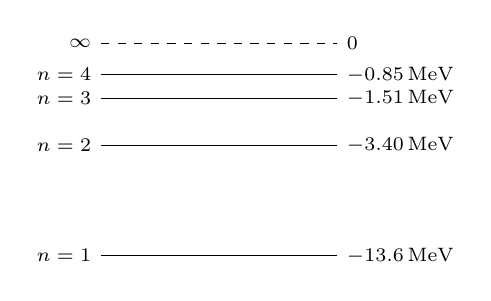
\begin{tikzpicture}[font=\scriptsize]
    \draw[dashed] (0,-.6)node[left]{\(\infty\)}--(3,-.6)node[right]{\(0\)};
    \foreach \y in {-3.3,-1.9,-1.3,-1}
        \draw (0,\y)--(3,\y);
    \foreach \y/\n in{-3.3/1,-1.9/2,-1.3/3,-1/4}
        \node at(0,\y)[left]{\(n =\n\)};
    \foreach \y/\n in{-3.3/-13.6,-1.9/-3.40,-1.3/-1.51,-1/-0.85}
        \node at(3,\y)[right]{\(\n\)\,\qty{}{MeV}};
\end{tikzpicture}